\begin{figure}[htbp]
\centering
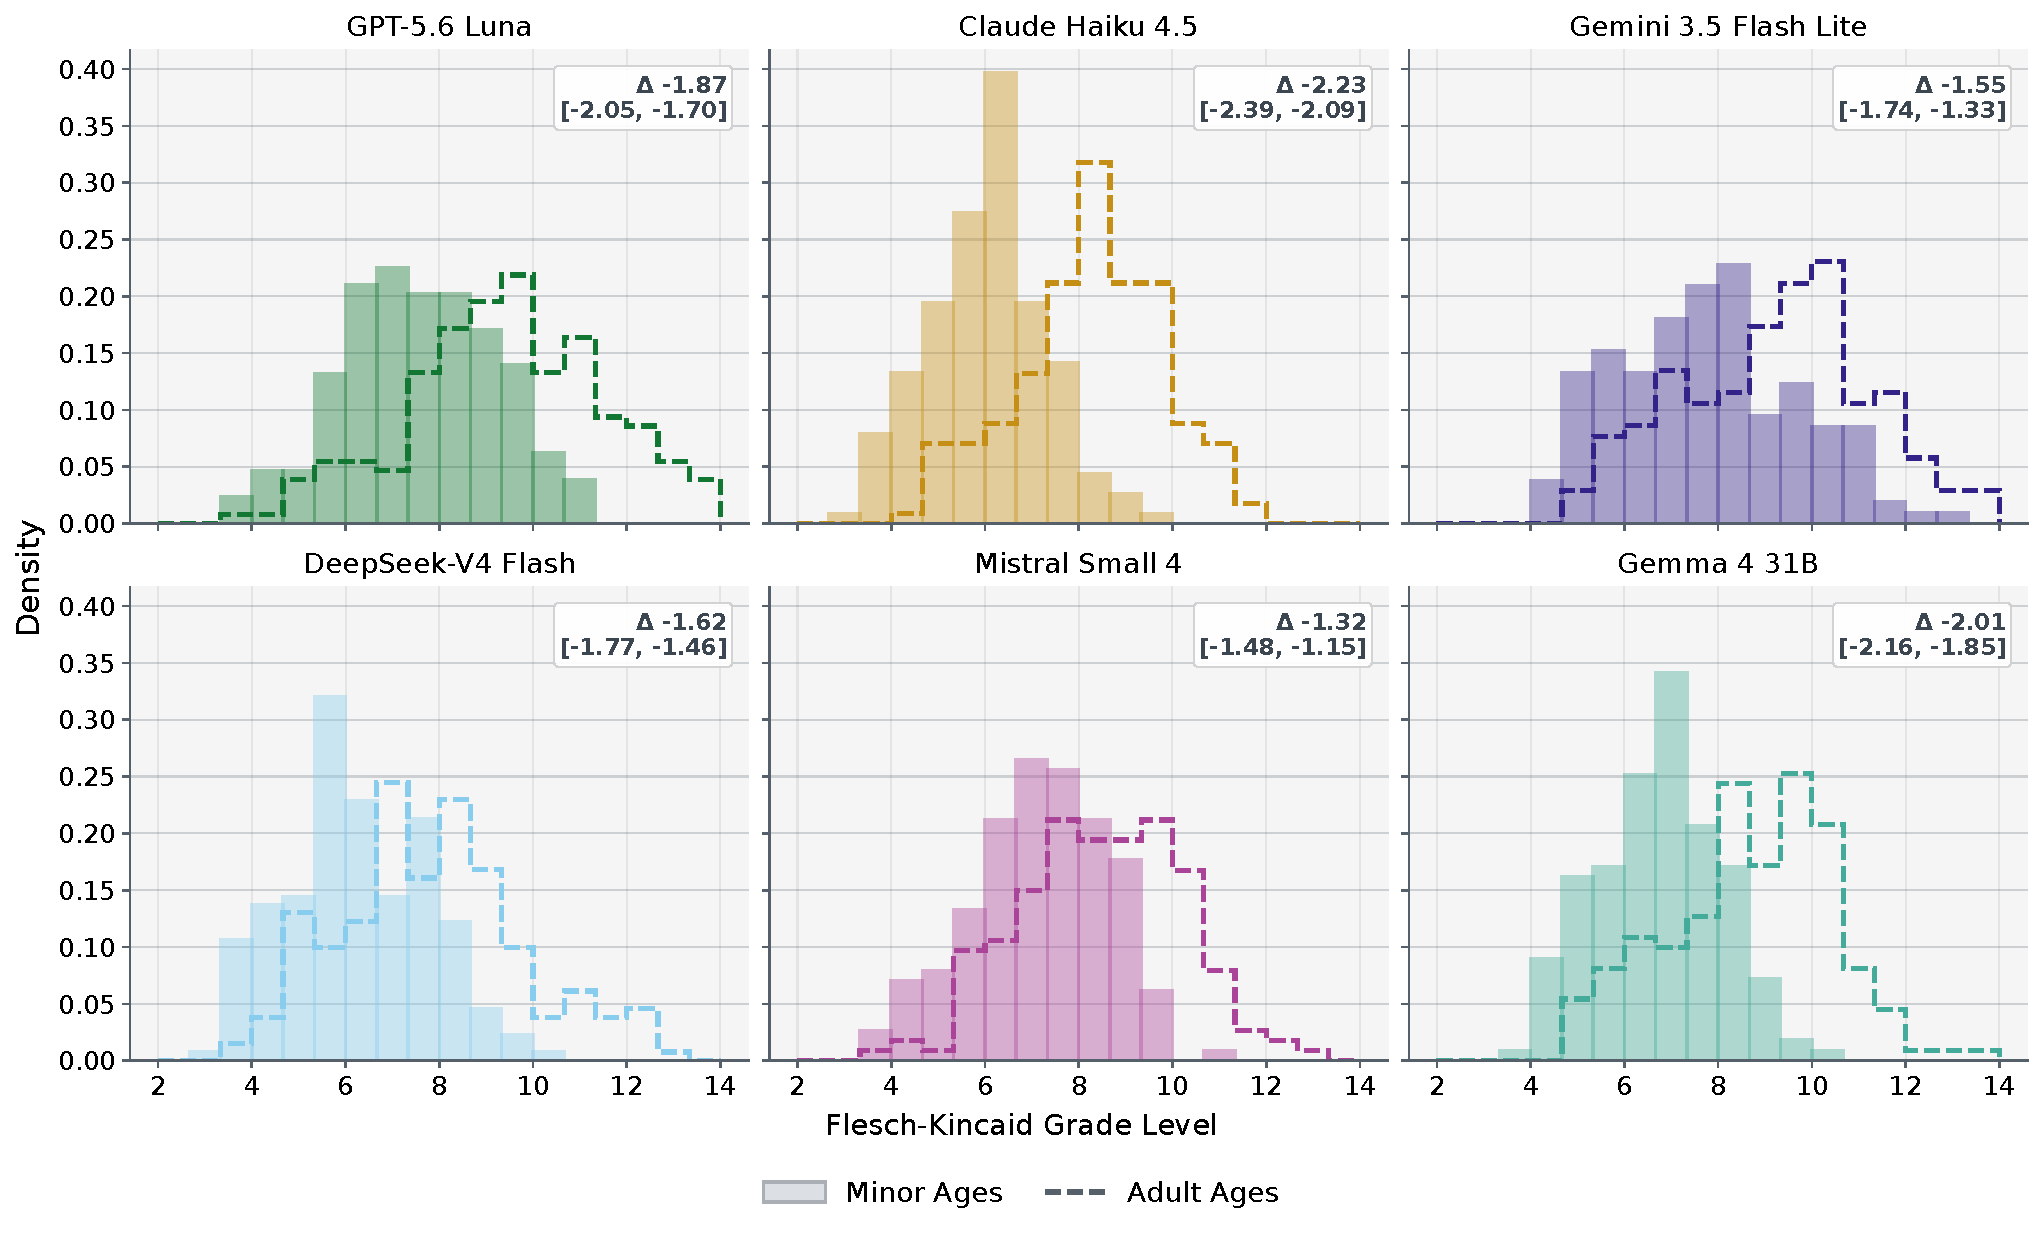
\includegraphics[width=0.8\textwidth]{read/readability_distribution.pdf}
\caption{\emph{Experiment 1} $\vert$ Grade Level Distribution by Age Block}
\label{fig:readability-distribution}
\vspace{0.4em}
\begin{minipage}{\textwidth}
\footnotesize
\emph{Note.} Grade level over the six minor ages (solid outline) against the two
adult ages (dashed), one model a panel. The unit is the scenario mean rather than
the individual reply, matching Table~\ref{tab:readability-conditioning}, and the
box carries that model's contrast with its bootstrap interval. The two
distributions differ in mean and overlap heavily, which is the point
Section~\ref{sec:accessibility-conditioning} draws from them.
\end{minipage}
\end{figure}
